\subsection{Aprendizado de Máquina}

Segundo \citeonline{directions_ia_ml_dp}, aprendizado de máquina é uma subcategoria de inteligência artificial que se refere  a detecção de padrões importantes de uma base de dados. As ferramentas utilizadas aumentam a eficiência dos algoritmos para lidar com bases de dados grandes.

Portanto, essa técnica permite ao computador melhorar os resultados com base na experiência, isso indica uma relação direta entre o quanto o programa consumiu de dados e qualidade da solução do problema \cite{ml_explicado}. 

Dentro desse nicho existem outros como: redes neurais, algoritmos evolucionários, algoritmos de busca, aprendizado por reforço, dentre outros. \cite{ml_oil_gas_industry}.

Existe relação direta de conceitos entre inteligência artificial, aprendizado de máquina e ciência de dados conforme mostrado na \cref{fig:diagrama_ia}.

\begin{figure}[H]
	\caption{Diagrama de Venn com aprendizado de máquina}
	\centering % para centralizarmos a figura
	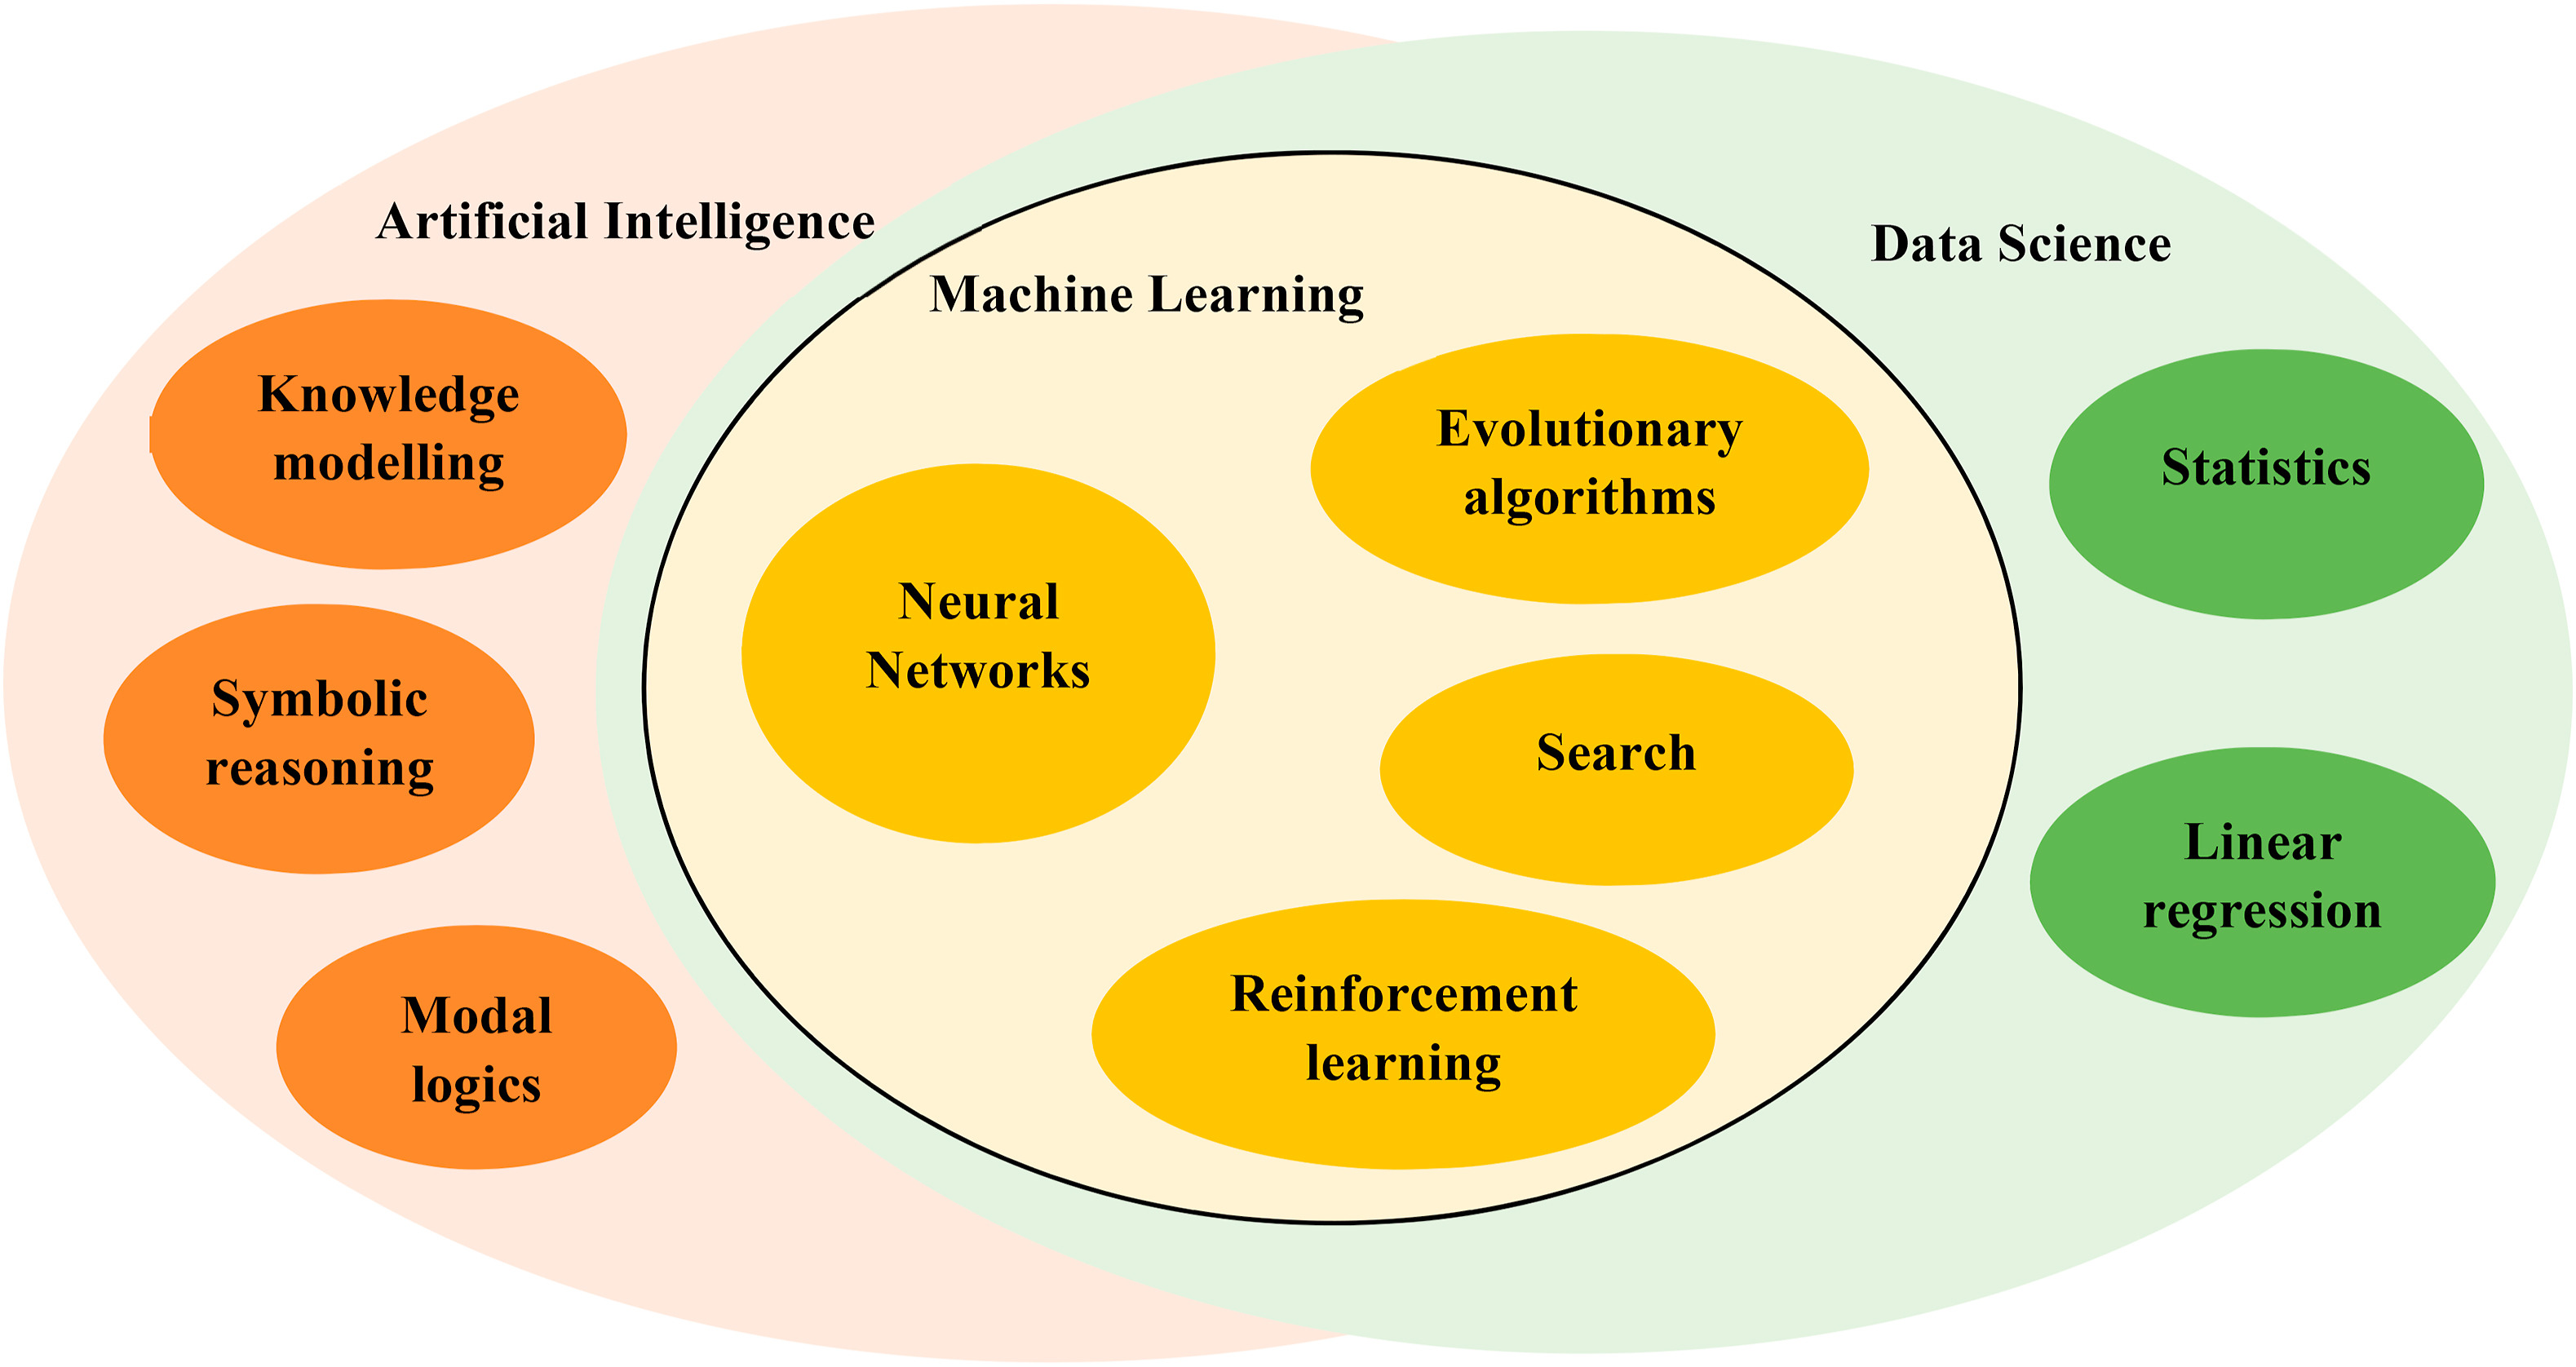
\includegraphics[width=10cm]{figures/diagrama_ia.jpg} % leia abaixo
	\legend{Fonte: \citeonline{ml_oil_gas_industry}}
	\label{fig:diagrama_ia}
\end{figure}

É possível observar uma hierarquia entre aprendizado de máquina e os principais termos sendo eles redes neurais artificiais e aprendizado profundo com base em \citeonline{ml_and_dp} mostrado no diagrama da \cref{fig:diagrama_ann}.

\begin{figure}[H]
	\caption{Ilustração da relação entre os principais tópicos de aprendizado de máquina}
	\centering % para centralizarmos a figura
	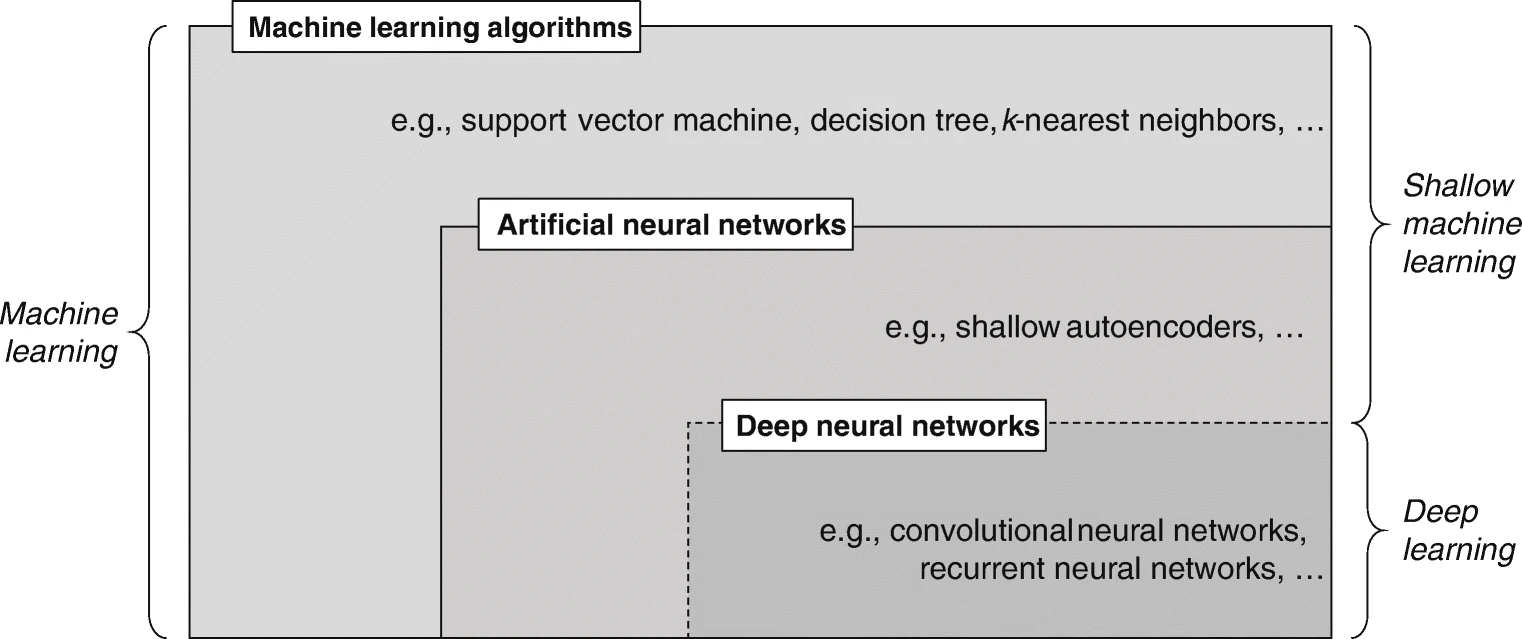
\includegraphics[width=10cm]{figures/diagrama_ann.jpg} % leia abaixo
	\legend{Fonte: \citeonline{ml_and_dp}}
	\label{fig:diagrama_ann}
\end{figure}
